\subsection{Операционные системы. Управление оперативной памятью в вычислительной системе. Алгоритмы и методы организации и управления страничной оперативной памятью.}

\textbf{Операционная система} --- комплекс программ, используемых для управления ресурсами компьютера и предоставления интерфейса пользователю.
В понятие управление ресурсами входит \textit{выделение} ресурсов для программ (например, памяти и процессорного времени),
\textit{защита} от доступа программ к ресурсам, которыми они не владеют, а также
\textit{абстрагирование} от оборудования, например, предоставление общего интерфейса для похожих типов устройств
(общий файловый интерфейс для всех дисков) или реализация виртуальных ресурсов (увеличение эффективного объема памяти за счет файла подкачки).


%\textbf{Операционная система} -- комплекс программ, в функции которого входит обеспечение контроля за существованием, использованием и распределением ресурсов вычислительной системы. 
%\textbf{Контроль за существованием ресурсов} -- обеспечение ОС реализации виртуальных ресурсов и предоставление средств доступа к физическим ресурсам. 
%\textbf{Использование ресурсов} -- ОС предоставляются все средства, обеспечивающие доступность ресурсов ВС пользователю (программам). \todo{мы с колей считаем, что определение всратое. ЖЕНЯ ПОМОГИ}
%\textbf{Распределение} -- выбор стратегии распределения и обеспечение всевозможных моделей регламентации доступа. 
% Фу, машбук

\textbf{Основные функции ОС}: 

- \textbf{Управление процессами} -- проблемы формирования процессов, поддержание жизненного цикла процесса, проблемы организации взаимодействия процессов, работа процессов с ресурсами.
    
- \textbf{Управление оперативной памяти} -- выбор стратегии организации ОП (реализация поддержки аппарата виртуальной памяти), защита ОП от несанкционированного доступа, задачи корректности работы процесса с выделенной ему ОП. 

- \textbf{Планирование} -- распределение времени центрального процессора, организация и обработка очередей обмена(решается проблема конкуренции доступа к устройству), обработка прерываний. 

- \textbf{Управление внешними устройствами и файловой системой}. Файловая система рассматривается, как виртуальное устройство. Подразумевается способ обмена в частности ввода и вывода данных в ВС, которая подразумевает использование буфера для временного хранения данных. 

- \textbf{Обеспечение сетевого взаимодействия} -- ОС должна обеспечивать функционирование и реализацию сетевых протоколов.

- \textbf{Обеспечение безопасности} -- устойчивость системы к возможным атакам, анализ функционирования системы и выявление попыток вторжения в систему. 


См. типы ос + базовая архитектура -- основная часть билет № 18

\textbf{Оперативное запоминающее устройство (ОЗУ)} -- устройства для хранения данных, в котором находится исполняемая в данный момент программа. Управление оперативной памятью включает в себя решение четырех задач: 
\begin{itemize}
    \item Контроль использования ресурсов - учет состояния каждой доступной в системе единицы памяти.
    \item Cтратегия распределения памяти - какому процессу, в течение какого времени и в каком объеме выделять соответствующий ресурс.
    \item Конкретное выделение ресурса тому или иному потребителю - для предоставляемого ресурса идет корректировка системных данных, а затем выдача его потребителю. 
    \item Освобождение памяти - окончательное освобождение памяти, происходящее в случае завершения процесса + освобождение памяти - задача принятия решения в случае, когда встает потребность высвободить физическую память из-под какого-то процесса за счет откачивания во внешнюю память, чтобы на освободившееся пространство поместить данные другого процесса. 
\end{itemize}  

\textbf{Существует несколько моделей по управлению ОП}:
\begin{itemize}
    \item Одиночное непрерывное распределение -- все адресное пространство разделяется на два компонента: в одной части располагается и функционирует операционная система, вторая часть отводится для выполнения прикладных процессов. Для разделения используется регистр границы - если получаемый исполнительный адрес оказывается меньше значения этого регистра, то это адрес пространста ОС, иначе - пространства процесса. 
    \item Распределение неперемещаемыми разделами -- все адресное пространство делится на две части: одна часть отводится под ОС, остальная - делится на N частей (разделов) и определяется под работу прикладных процессов. Два варианта распределения процесов: обща очередь и очередь к каждому разделу. Необходимо использовать два регистра границ - регситры, отвечающие за начало области и ее конец или механизм ключей защиты, которые могут находиться в слове состояния процесса и в слове состояния процессора. При обращении к памяти совпали — доступ разрешен.
    \item Распределение перемещаемыми разделами. Исполняемый код процесса может перемещаться по оперативной памяти. Локальная компрессия - система для высвобождения памяти передвигает небольшое количество процессов. Глобальная компрессия - система приостанавливает работу всех процессов и начнает их перемещать, например,  к начальному адресу ОЗУ, так, вся свободная память - в конце ОЗУ. Используются аппаратные средства защиты памяти - регистры границ или ключи защиты, для перемещения используют регистр базы. Избавляет от фрагментации. 
    \item Страничное распределение. Все адресное пространство -- совокупность блоков фиксированного размера, которые называются \textbf{страницами}. \textbf{Виртуальное адресное пространство} - пространство с адресами которого оперирует программа. \textbf{Физическое адресное пространство} - пространство, которое есть в наличие в компьютере. 
    \item Сегментное распределение -- каждый процесс -- совокупность сегментов определенного размера: сегмент кода, сегмент стат. данных, сегмент стека. ]Используется некоторая таблица, в которой хранится информация о каждом сегменте - его номер, размер и тд. Виртуальный адрес интерпретируется, как номер сегмента и величина смещения в нем. 
\end{itemize}

\textbf{Страничное распределение}. Устанавливается соответствие между виртуальными и физическими страницами. Для преобразования виртуального адреса в физический используется таблица страниц. Типовая структура записи таблицы страниц содержит информацию о номере физической страницы, а также совокупность атрибутов, например, флаг модификации содержимого страницы, присутствие/отсутствие страницы и другие. 
\begin{itemize}
    \item Использование TLB-таблиц. Виртуальный адрес = номер виртуальной страницы + адрес смещения в ней. Если промах - выкидывается самая старая страница и добавляется новая. 
    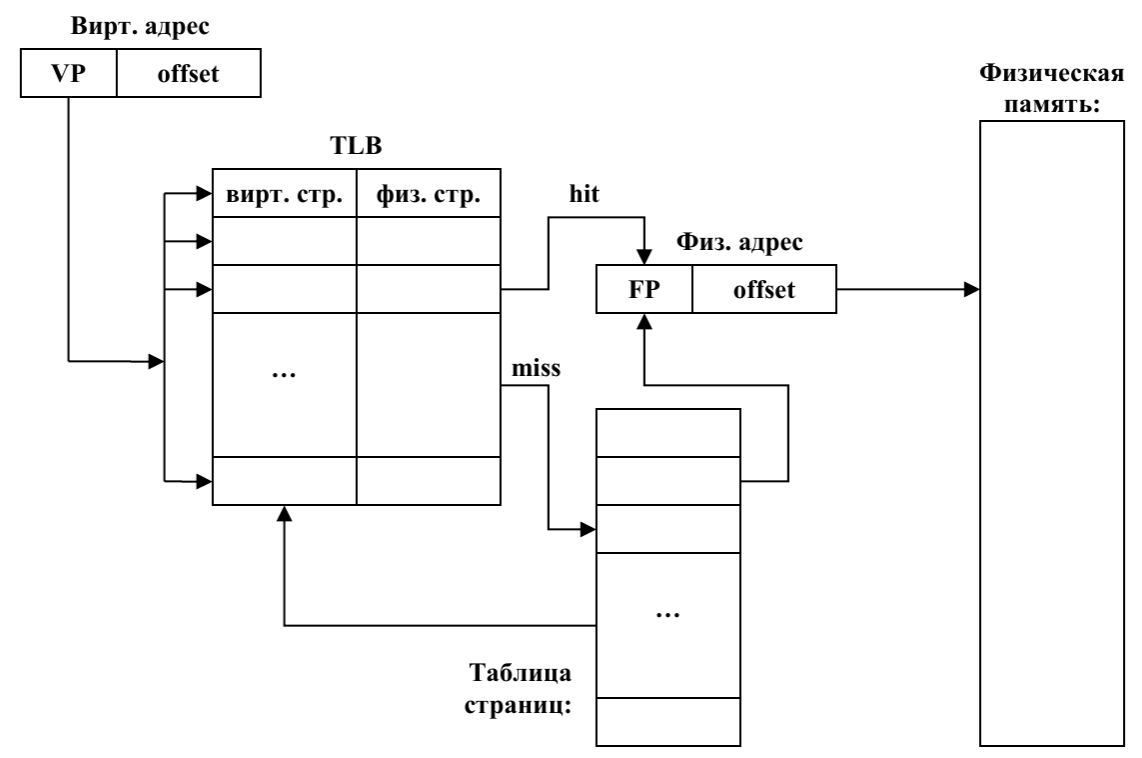
\includegraphics[width=\columnwidth]{pics/tlb.png}
    \item Иерархическая организация таблиц страниц. Информация о странице представляется в виде совокупности номеров, используя которые, можно получить номер соответствующей физической страницы. 
    \item Хеширование. Извлекается номер виртуальной страницы, который подается в хэш-функцию, отображающей значение на аппаратную таблицу фиксированного размера. Каждая ее запись - список коллизий, каждая из них - пара вирт. стр + физ. стр.  
    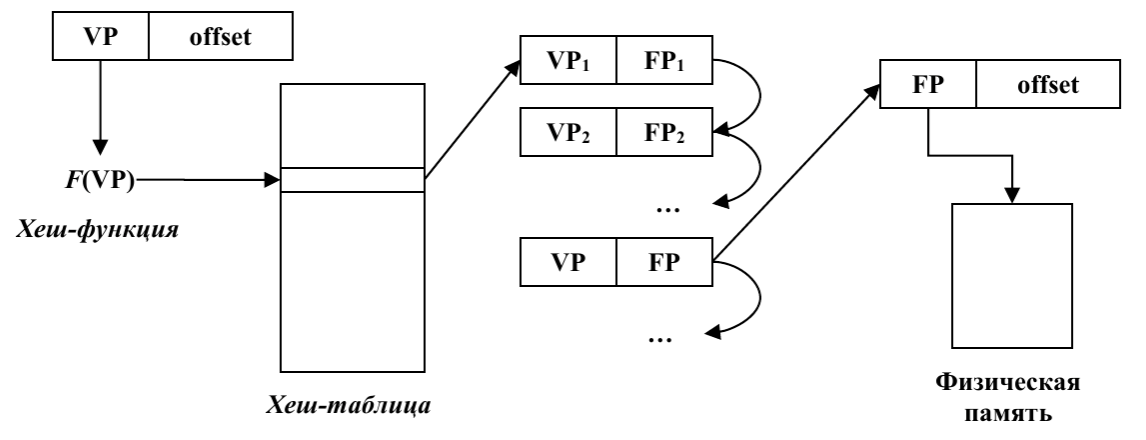
\includegraphics[width=\columnwidth]{pics/hash.png}
    \item Инвертированные таблицы страниц. Виртуальный адрес = PID + номер вирт. стр. + смещение. Номер строки в таблице -- адрес физической таблицы.
    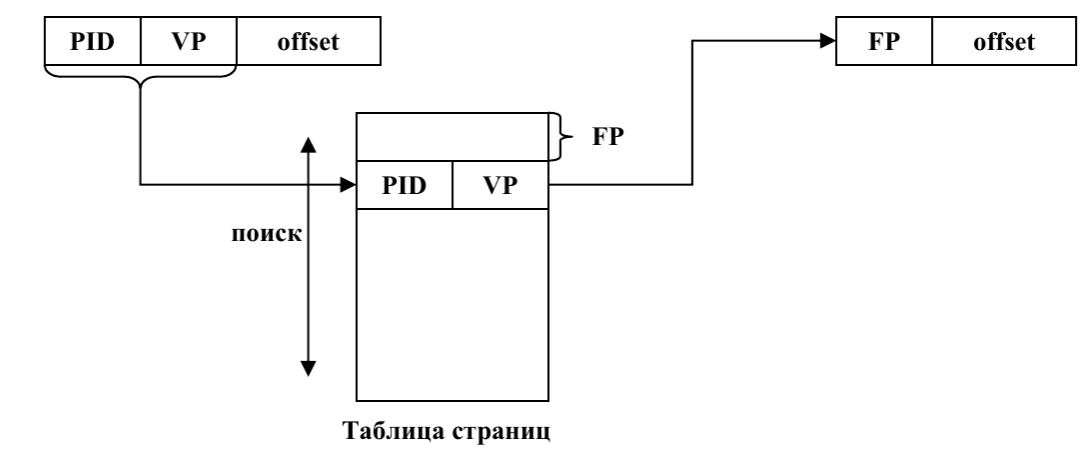
\includegraphics[width=\columnwidth]{pics/inv.png}
\end{itemize}


% -------- source --------
\bigbreak
[\cite[page 69-96]{replace_me}]